\documentclass[tikz,border=10pt]{standalone}

\usepackage{amsmath}
\usetikzlibrary{arrows.meta,positioning}

\begin{document}

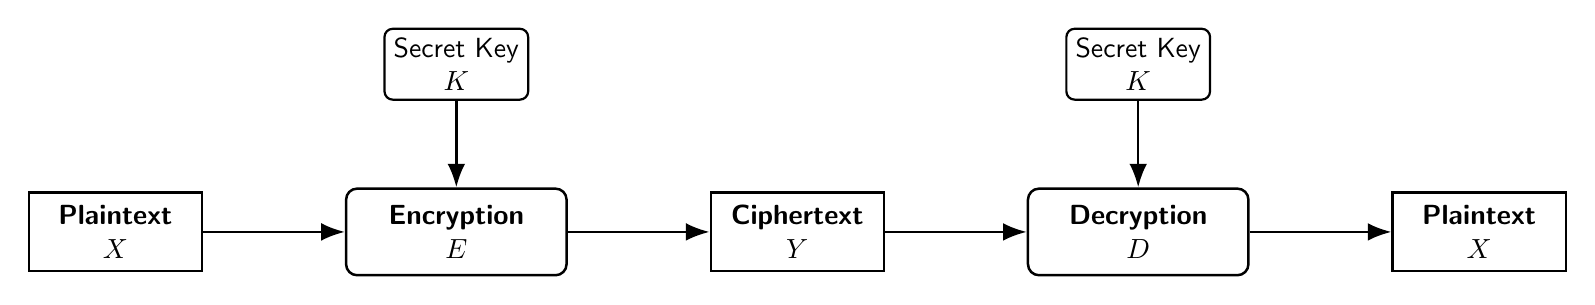
\begin{tikzpicture}[
    font=\sffamily,
    node distance=1.8cm,
    box/.style={
        draw,
        rounded corners=4pt,
        minimum width=2.8cm,
        minimum height=1.1cm,
        align=center,
        line width=0.9pt
    },
    data/.style={
        draw,
        minimum width=2.2cm,
        minimum height=1.0cm,
        align=center,
        line width=0.8pt
    },
    key/.style={
        draw,
        rounded corners=3pt,
        minimum width=1.8cm,
        minimum height=0.8cm,
        align=center,
        line width=0.8pt
    },
    arrow/.style={
        -{Latex[length=3mm]},
        line width=0.9pt
    }
]

\node[data] (plain1) {
    \textbf{Plaintext}\\
    $X$
};

\node[box, right=of plain1] (enc) {
    \textbf{Encryption}\\
    $E$
};

\node[data, right=of enc] (cipher) {
    \textbf{Ciphertext}\\
    $Y$
};

\node[box, right=of cipher] (dec) {
    \textbf{Decryption}\\
    $D$
};

\node[data, right=of dec] (plain2) {
    \textbf{Plaintext}\\
    $X$
};

\node[key, above=1.1cm of enc] (key1) {
    Secret Key\\
    $K$
};

\node[key, above=1.1cm of dec] (key2) {
    Secret Key\\
    $K$
};

\draw[arrow] (plain1) -- (enc);
\draw[arrow] (enc) -- (cipher);
\draw[arrow] (cipher) -- (dec);
\draw[arrow] (dec) -- (plain2);

\draw[arrow] (key1) -- (enc);
\draw[arrow] (key2) -- (dec);

\end{tikzpicture}

\end{document}